\documentclass[../TST.tex]{subfiles}
\begin{document}
\begin{eproblem}[N-resistor black box]{\ \\[5pt]}
\textit{Equipment:}\\
Sealed paper box with a closed circuit (Figure \ref{fig2}), multimeter, ruler, graph paper. The circuit consists of $N$ identical resistors in series, each of resistance $R_0$. You can only access the terminals of 12 adjacent resistors.
\begin{figure}[h]
		\centering
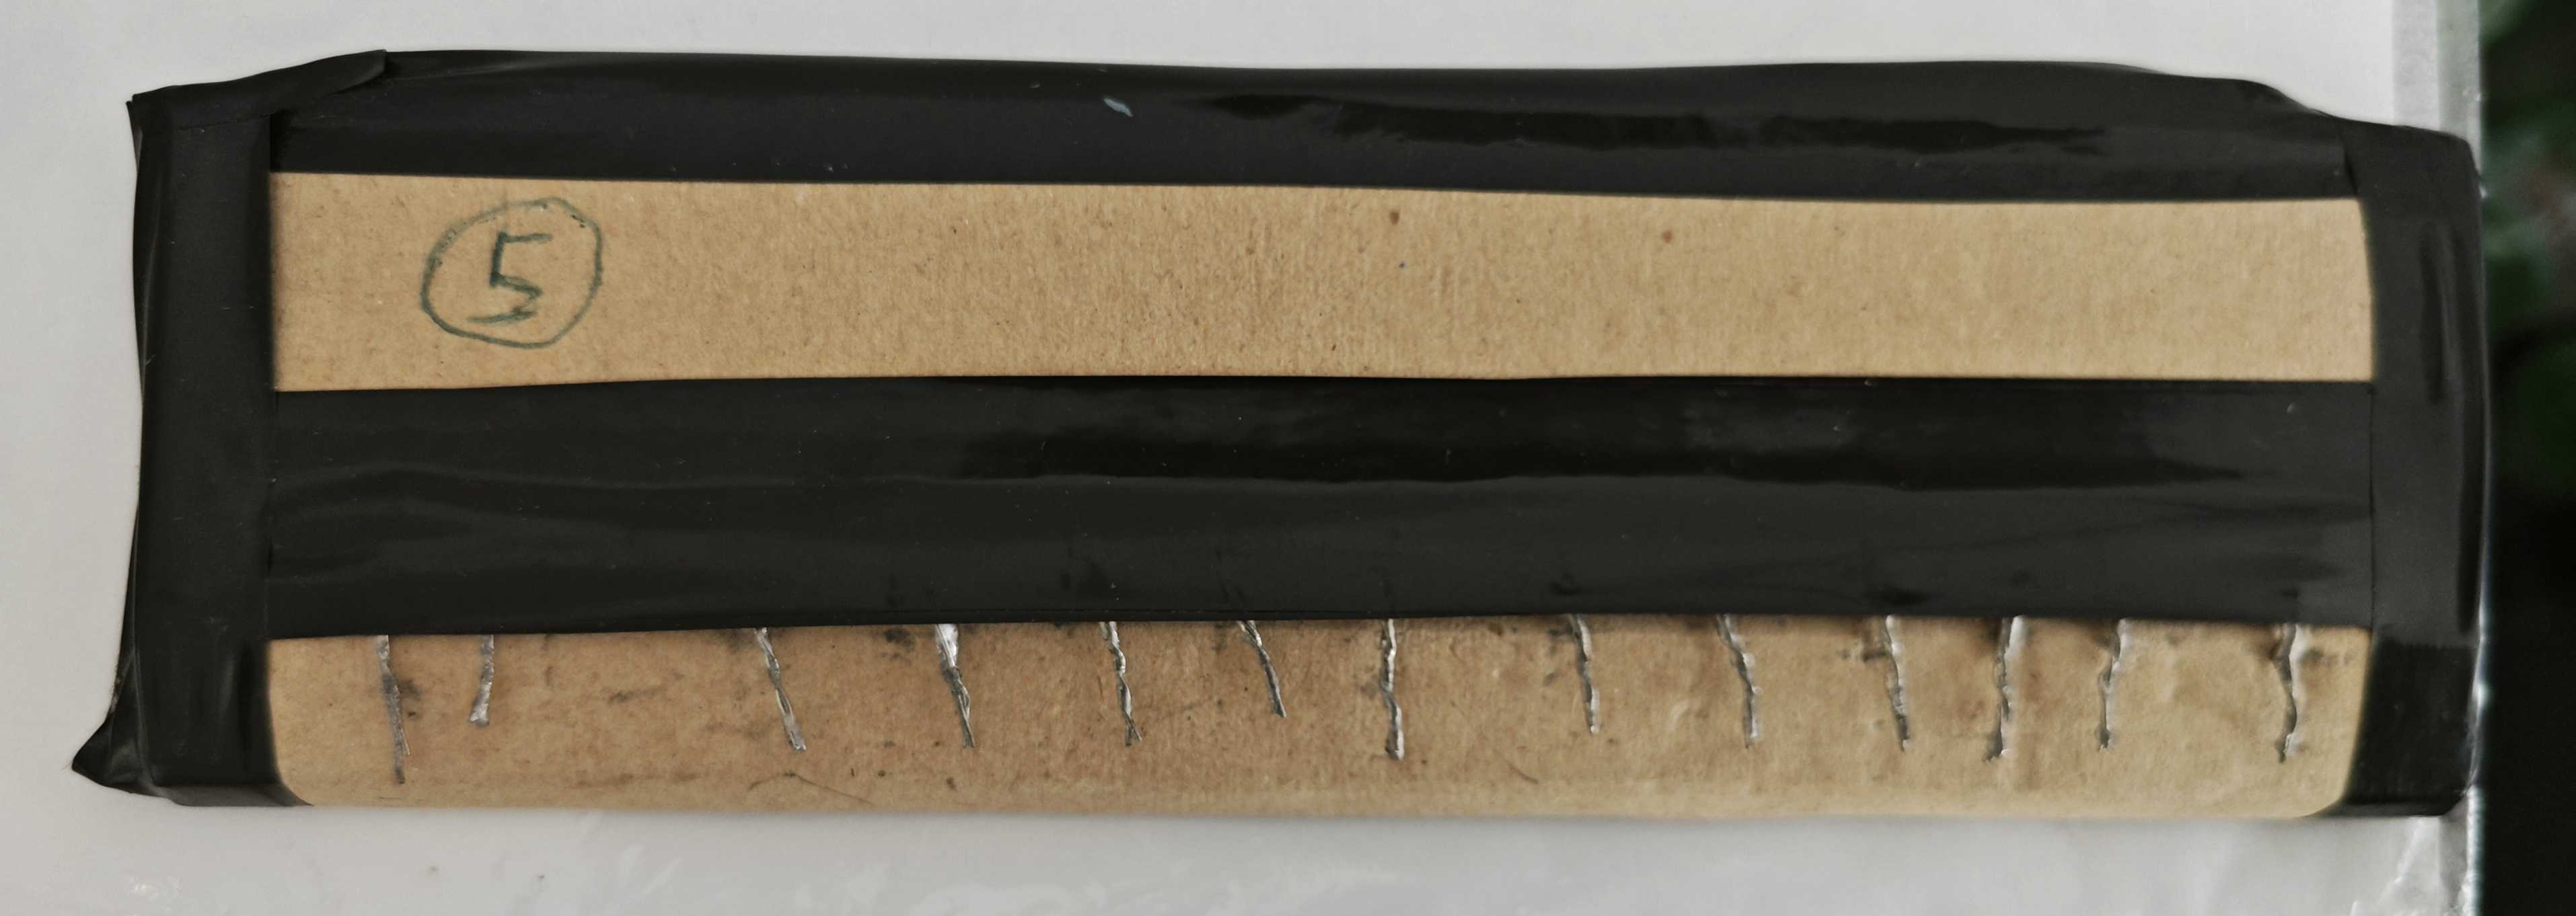
\includegraphics[width=0.6\textwidth]{fig/2010_e1.jpg}
    \caption{}
	\label{fig2}
\end{figure}

The aim of this problem is to find the resistance $R_0$ and the number of resistors in the box $N$.
\begin{subpart}
	\item Find a formula for the resistance $R(k)$ of the circuit when measuring between terminals which are $k$ resistors away from each other.\score{1.0}
	\item Describe a method for finding the resistance $R_0$ and the number of resistors $N$ by plotting a series of measurements.\score{1.0}
	\item Take the necessary measurements. Present them in a table and explain how they were obtained. \score{3.0}
	\item State the variables which, when plotted, can easily give you $R_0$ and $N$. \score{1.0}
	\item Plot the relevant graph. \score{4.0}
	\item Using the graph, determine $R_0$. \score{1.5}\\
		Likewise, determine $N$. \score{2.5}
	\item Estimate your error in finding $R_0$. \score{0.5}\\
		Estimate your error in finding $N$. \score{0.5}
\end{subpart}
Call the examiner in case of any technical difficulties.\\

\textbf{Note:} If there is evidence that the box has been unsealed or that the circuit has been interrupted, you will be disqualified.  
\end{eproblem}
\end{document}
